\documentclass[10pt]{article}
\usepackage{ctex}
\usepackage{graphicx}
\graphicspath{{E:/大学课程/大一下/人工智能程序设计/作业集/第十四周作业/图片集/},{pics/}}
\usepackage{amsmath}
\usepackage{amssymb}
\usepackage{float}%使图片紧跟在文字后面

\title{第十四周问答作业}
\author{朱士杭\ 231300027}
\date{\kaishu \today}

\begin{document}
	\maketitle
	\section{问题一:电商数据预处理}
	具体见“第十四周问答作业.ipynb”
	\begin{figure}[H]
		\centering
		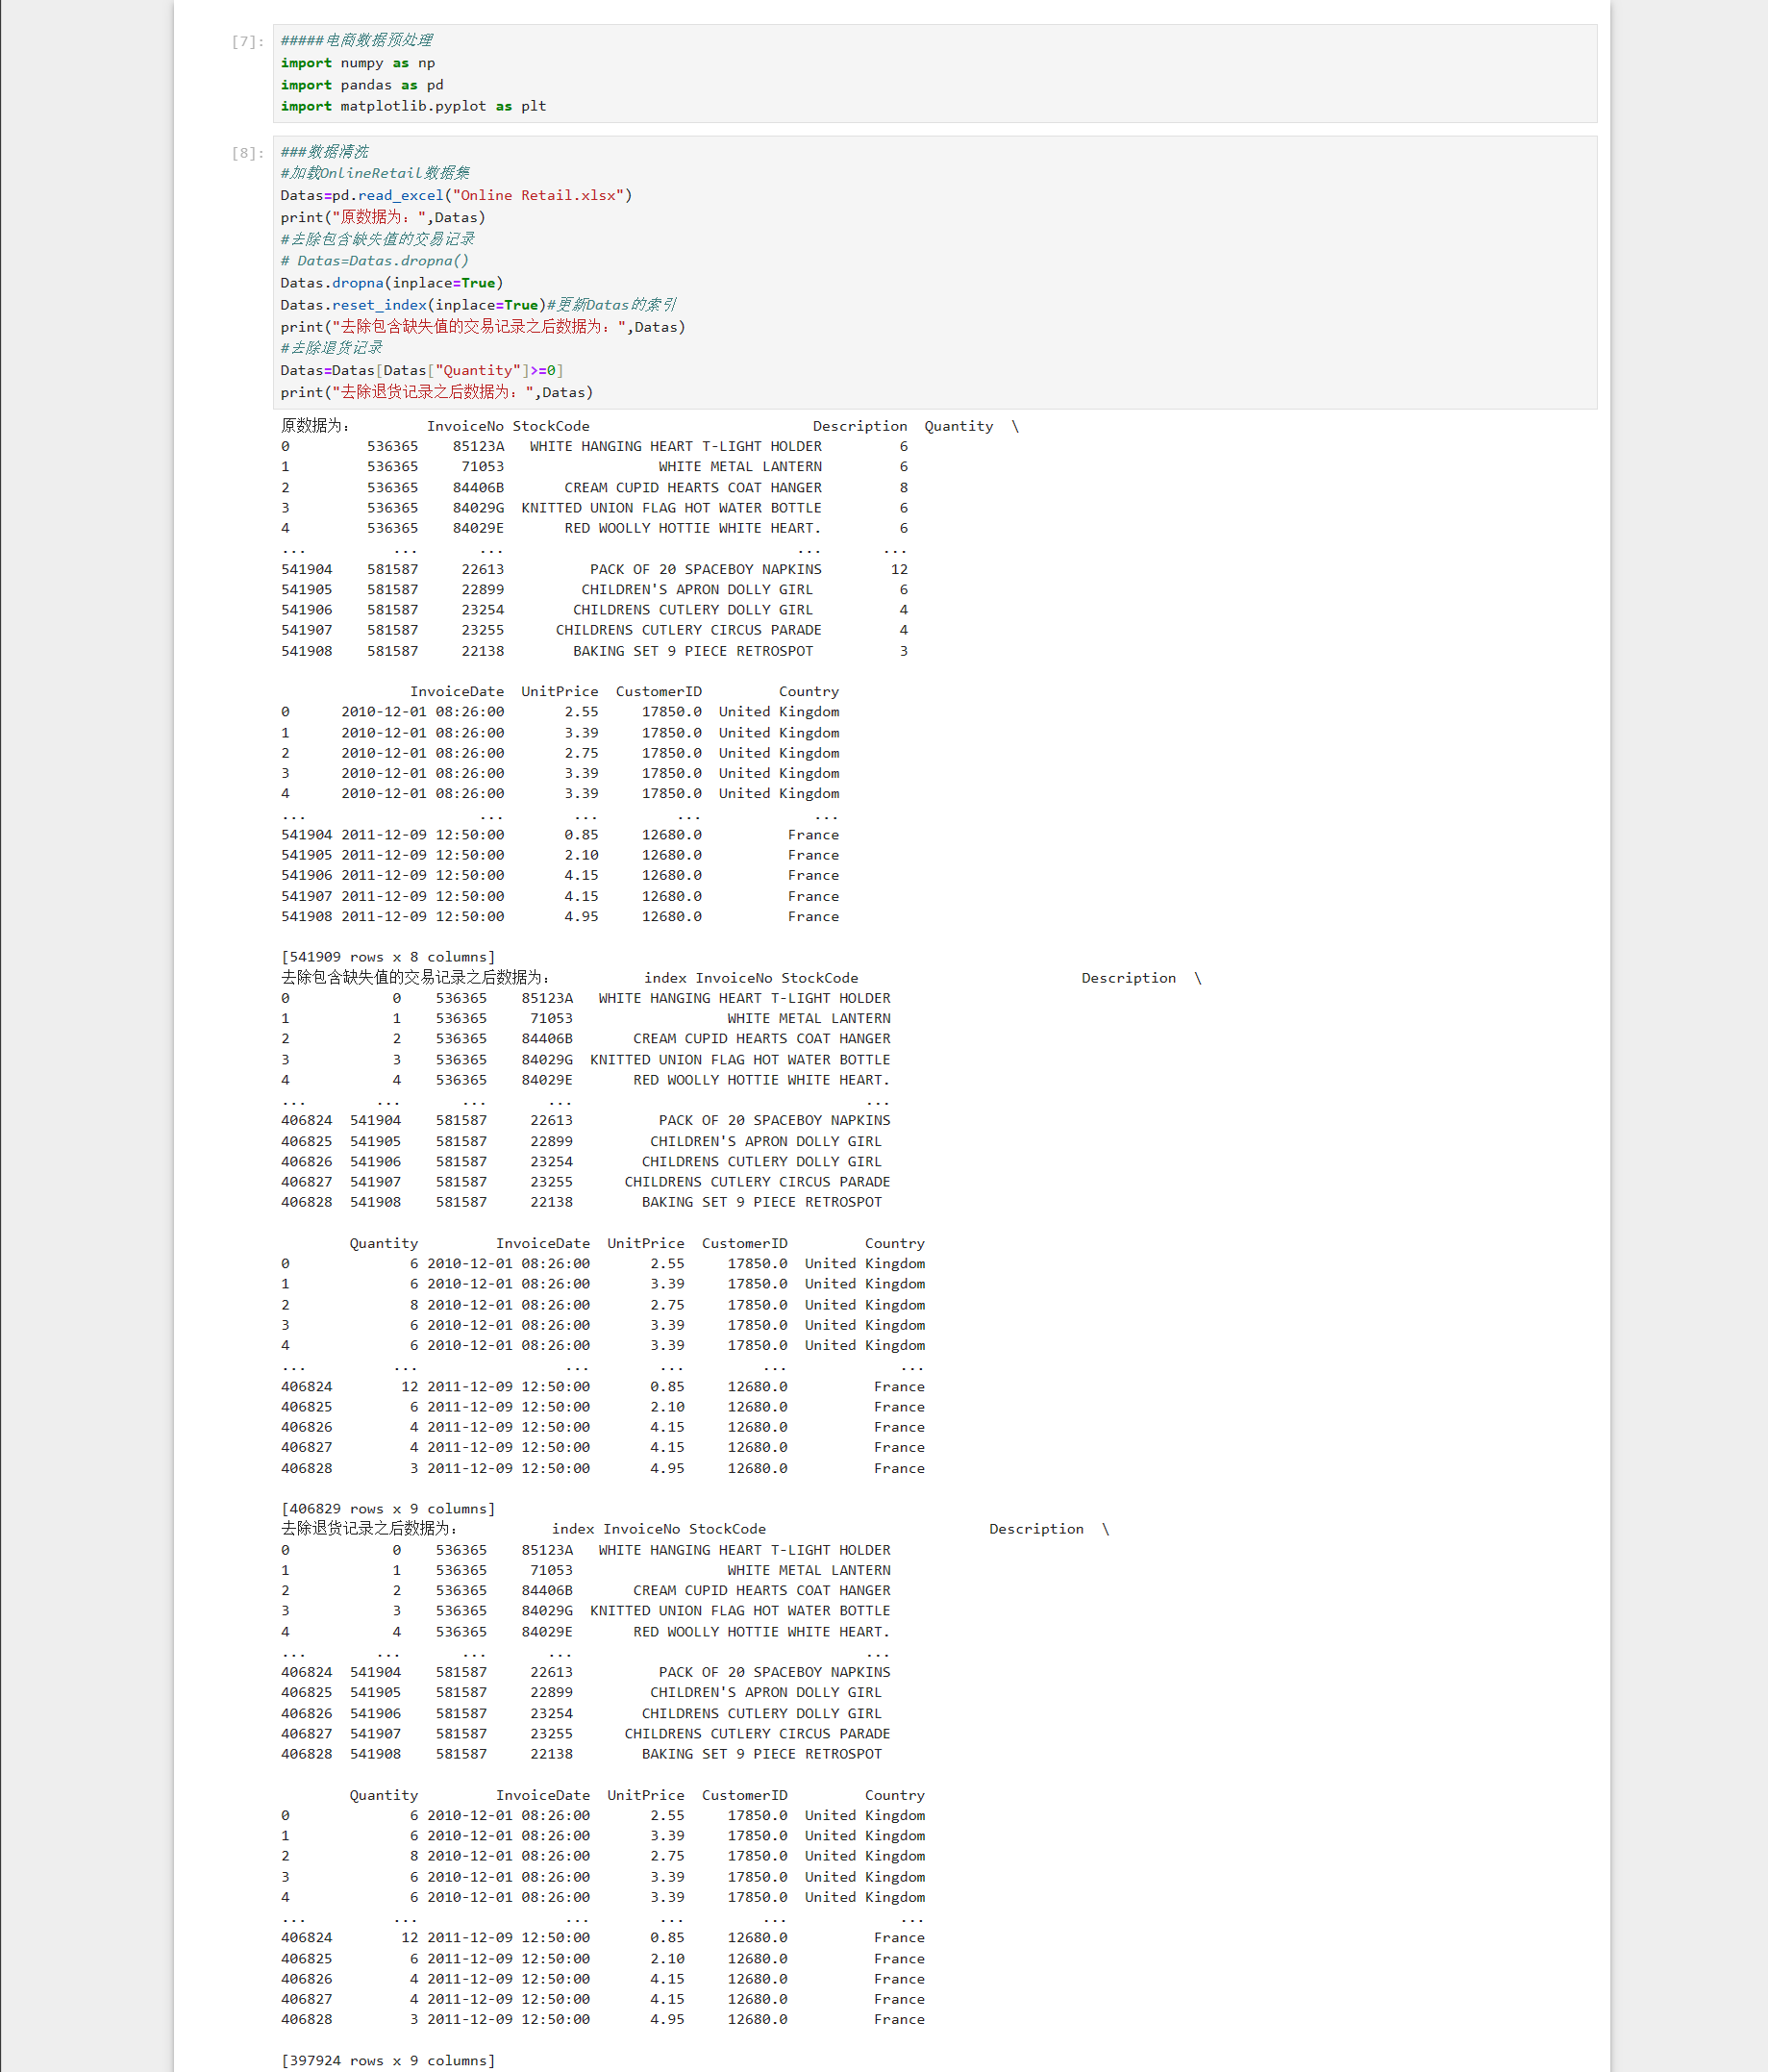
\includegraphics[scale=0.24]{1}
		\caption{电商数据清洗}
	\end{figure}
	\begin{figure}[H]
		\centering
		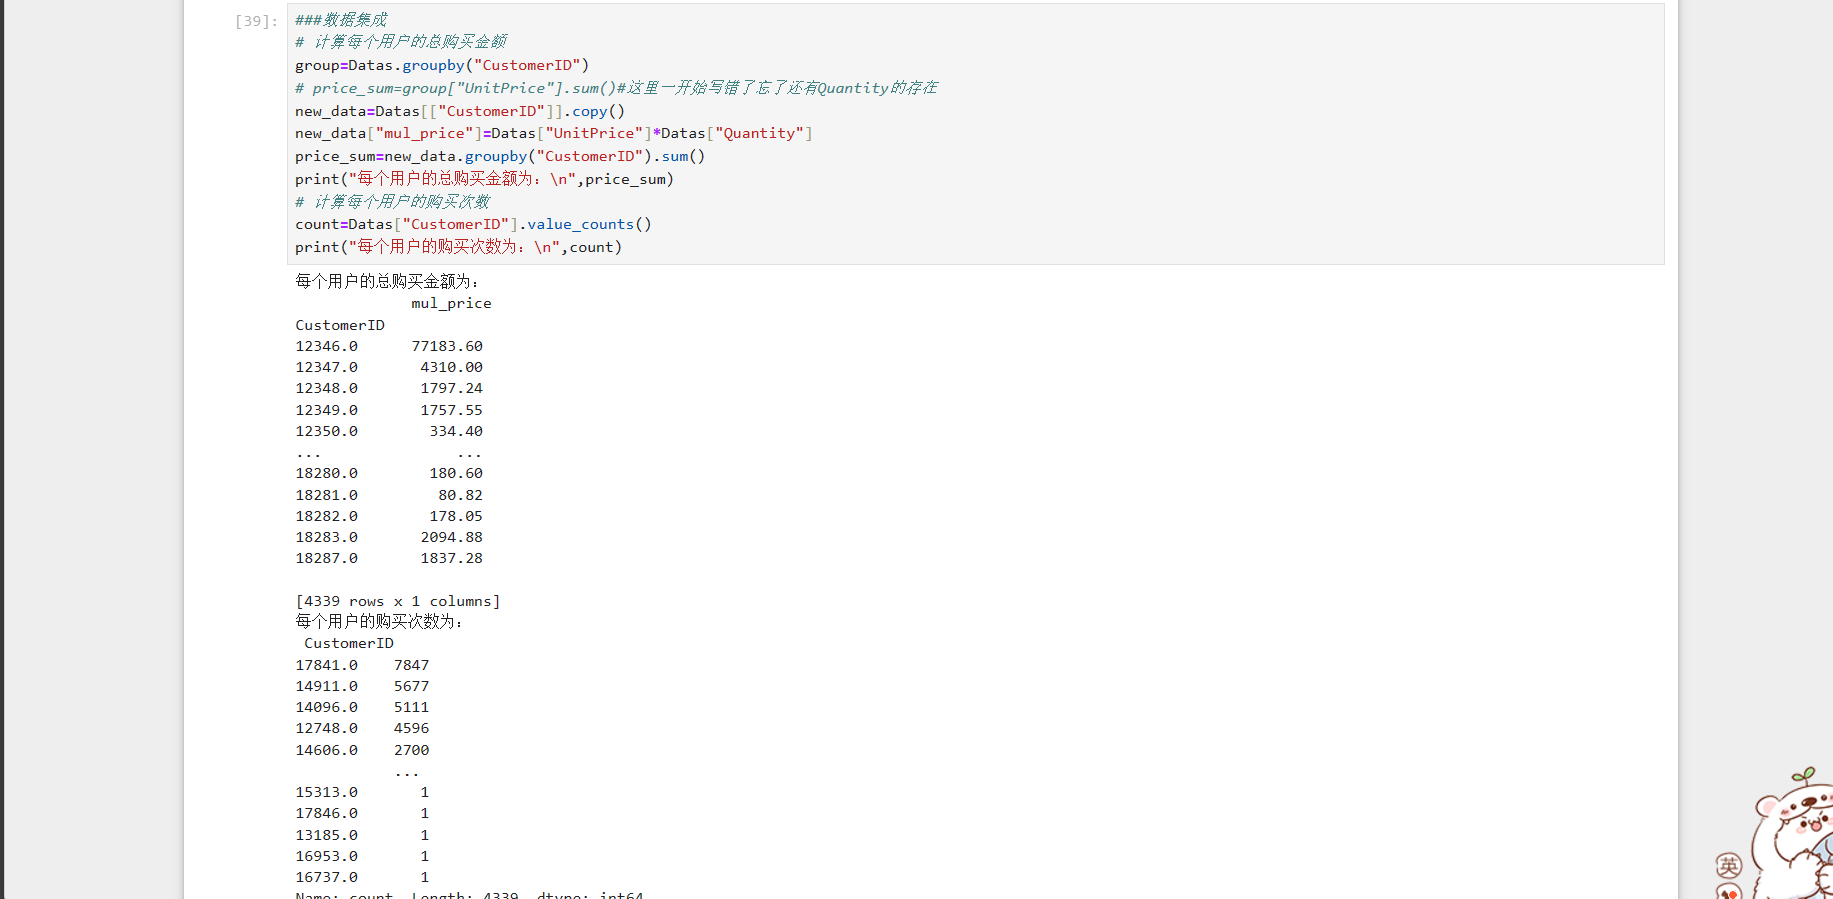
\includegraphics[scale=0.3]{3}
		\caption{电商数据集成}
	\end{figure}
	\begin{figure}[H]
		\centering
		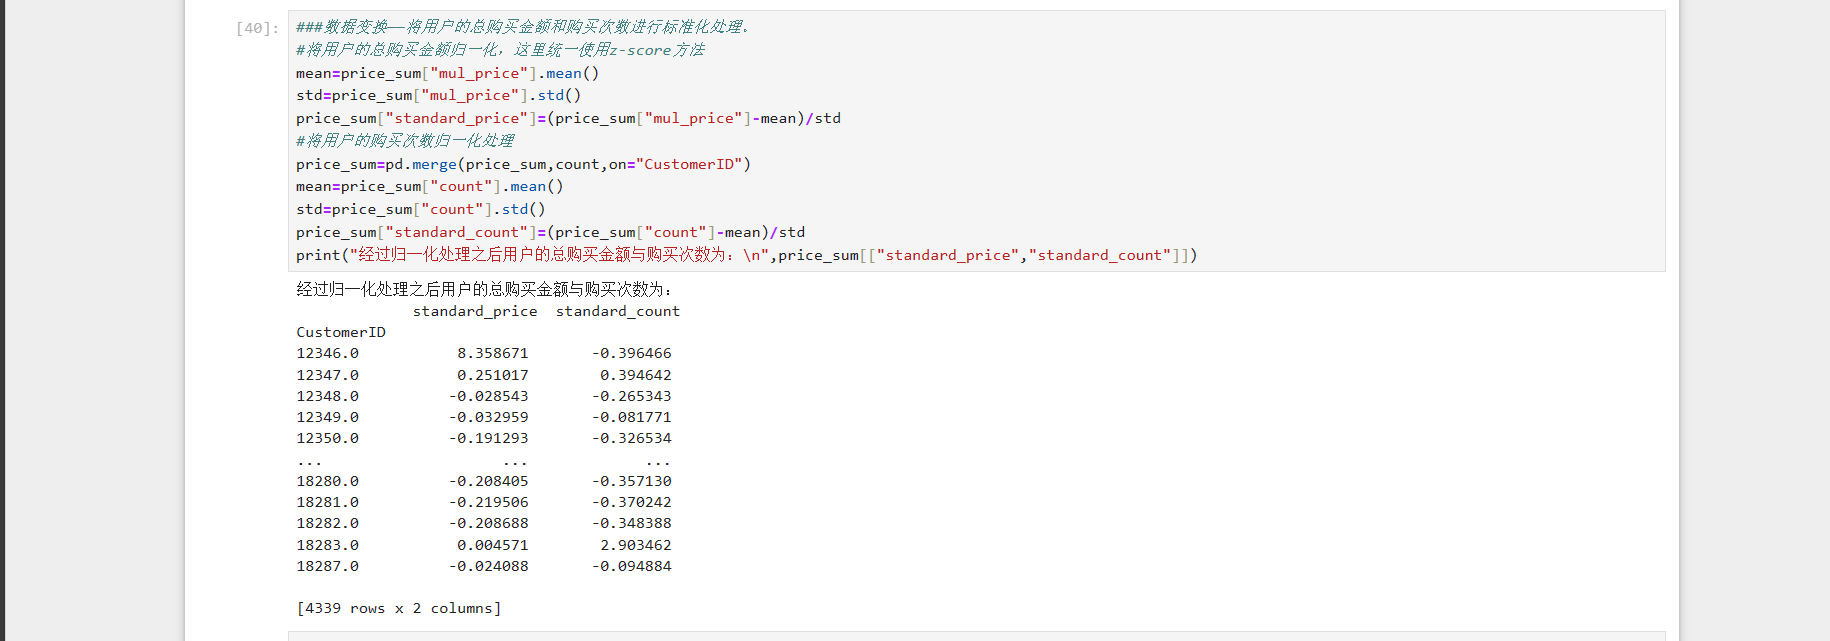
\includegraphics[scale=0.3]{4}
		\caption{电商数据变换}
	\end{figure}
	
	\section{问题二:为什么在PCA之前需要进行标准化处理}
	如果不进行标准化处理的话很有可能出现“大数吃小数”的现象,比如说$$( ( 100000 , 0.5 ) , ( 111000 , 0.55 ) , ( 99900 , 0.32 ) )$$
	这三个数据点,其实沿着y轴方向相对变化也是很大的,但是根据PCA的公式,第二维(y轴)的数据直接被“吃掉”了,
	而我们实际在比较的时候应当是相对分布而不是绝对分布,因此需要使用归一化的手段使得数据分布更加“公平”。
	
	\section{问题三:使用PCA对词向量进行降维和可视化}
	具体见“第十四周问答作业.ipynb”
	\begin{figure}[H]
		\centering
		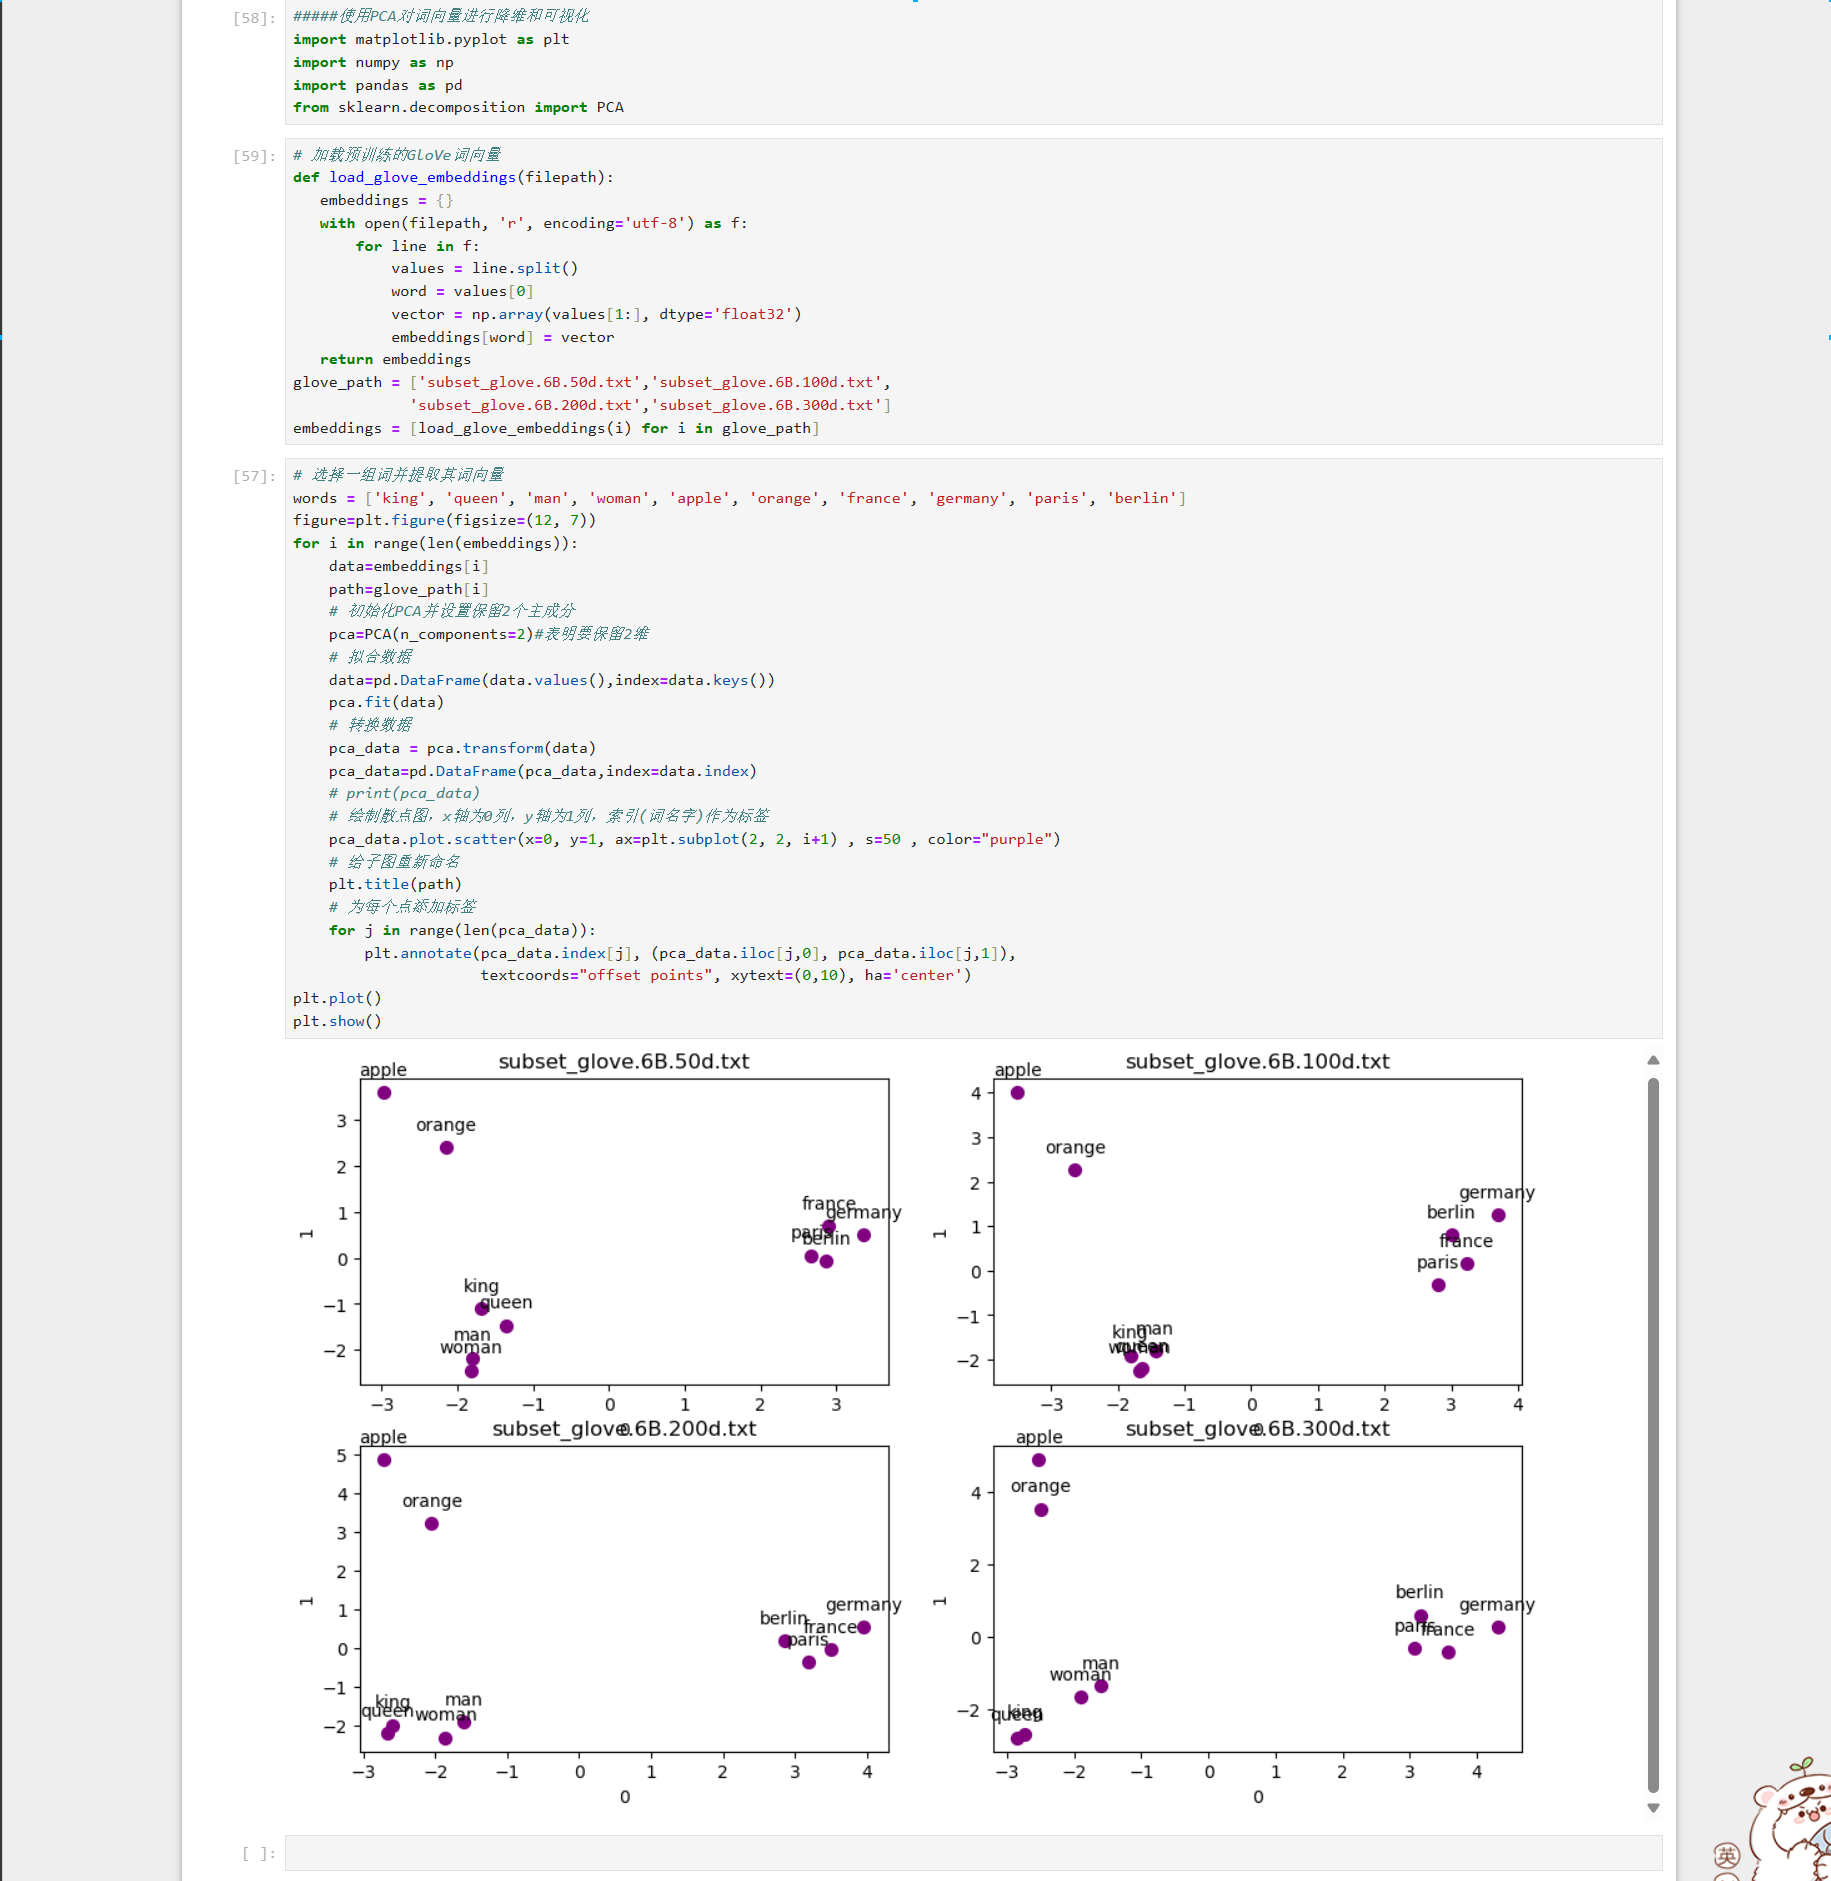
\includegraphics[scale=0.27]{2}
		\caption{PCA降维和可视化}
	\end{figure}
	
	
	\section{问题四:评估多元线性回归模型的性能}
	\subsection{如何评估性能}
	核心想法就是看最终的拟合效果如何,比如说我将原先的数据集分成3部分——训练集、测试集和验证集\par
	训练集用于生成多元线性回归模型,测试集用于测试模型误差并进行调优,而最终用验证集的数据去评估模型的性能如何,
	通过将输入数据投喂进去,然后得到最后的结果(标签)\par
	如果是回归任务,则比较和真正结果相差多少(方差);
	如果是分类任务,则求出分类的正确率即可
	
	\subsection{常用评估指标}
	\subsubsection{拟合优度(Goodness of Fit)}
	决定系数(R²)表示模型解释的变异性的比例,值越接近1说明模型解释能力越强\par
	调整后的决定系数(Adjusted R²)考虑到自变量数量的影响,当自变量增多时,R²往往会上升,调整后的R²对自变量的数量进行了惩罚,能更准确地反映模型的性能\par
	\subsubsection{F检验}
	用于检验模型整体是否显著,即至少有一个自变量对因变量有显著影响。
	\subsubsection{t检验}
	对每个回归系数进行检验,判断每个自变量是否对因变量有显著影响。
	\subsubsection{置信区间}
	每个回归系数的置信区间,如果置信区间不包括0,通常认为该系数是显著的
	\subsubsection{均方误差(MSE)}
	预测值与实际值之间差异的平方的平均数,MSE越小,说明模型的预测精度越高。\par
	另一种为均方根误差(RMSE)为MSE的平方根,它和因变量的量纲一致,更直观地反映了预测误差的大小。
	\subsubsection{交叉验证}通过将数据集分成多个部分,在不同的子集上训练和测试模型,来评估模型的稳健性和预测能力。
	\subsubsection{残差图}检查残差是否随机分布,如果残差图中存在明显模式(如曲线形状或扇形),则说明模型可能存在问题。\par
	另一种是标准化残差,将残差除以其标准差,用于检测异常值和模型的不稳定性。
	
	
	
	
	
	
	
	\section{问题五:比较对数几率回归(逻辑斯蒂回归)和KNN}
	\subsection{对数几率回归(Logistic Regression)}
	对数几率回归是一种广义线性模型,用于二分类或多分类问题。它通过使用逻辑函数(Logistic Function)将线性回归的输出映射到0和1之间的概率\par
	对数几率回归关注于找到特征和类别概率之间的最佳拟合,核心公式是使用一个连续可微的函数y=1/(1+exp(-wx+b))使得一个二分类函数映射到0-1之间\par
	训练阶段需要计算参数的梯度并更新,测试阶段对于新的数据点,计算其预测概率是快速的。\par
通常需要对特征进行缩放,并且可以加入正则化项(如L1或L2正则化)来防止过拟合\par
	当特征数量较多时,对数几率回归可以有效地进行特征选择和权重分配。它适用于数据量较大,特征维度较高,且需要解释模型的情况\par
	
	\subsection{K-最近邻(KNN)}
	KNN是一种基于实例的学习算法,它不需要显式地训练模型参数\par
	预测过程中KNN算法会在训练集中找到与待预测数据点最接近的K个数据点,并根据这K个邻居的类别进行投票来决定待预测点的类别。
	说白了就是找到跟想要预测的点最相似的K个点,再根据他们的类别少数服从多数\par
KNN适用于数据量较小,特征维度较低的情况。当数据分布不均匀或存在噪声时,KNN通过平均多个近邻的响应来减少误差。\par
	
	\subsection{异同点}
	\subsubsection{模型复杂度}对数几率回归在训练阶段有较高的计算复杂度,而KNN在测试阶段计算复杂度较高。
	\subsubsection{数据需求}对数几率回归需要较少的数据来训练模型参数,而KNN在训练阶段不需要数据来学习参数,但在预测时需要较多的数据来找到近邻。
\subsubsection{泛化能力}对数几率回归通过模型参数来泛化,而KNN通过训练数据来泛化。
	\subsubsection{可解释性}对数几率回归的参数可以直接解释为特征对类别概率的影响,而KNN没有显式的参数来解释。
\subsubsection{对异常值的敏感性}对数几率回归对异常值相对不敏感,因为它寻找的是全局最优解;而KNN对异常值非常敏感,因为异常值会影响近邻的选择。
	
	\subsection{适用场景选择}
	当数据量较大,特征维度较高,且需要模型具有较好的解释性时,优先选择对数几率回归。
	当数据量较小,特征维度较低,或者数据分布不均匀,噪声较多时,可以考虑使用KNN\par
	在实际应用中,通常需要根据具体问题和数据集的特点来选择合适的算法,并通过交叉验证等方法来评估和比较不同算法的性能。
	
	
	\section{分类模型对手写数字数据集分类}
	具体见“第十四周问答作业.ipynb”
	
\end{document}